\documentclass[a4paper,11pt]{article}
\usepackage{indentfirst}
\usepackage[T1]{fontenc}
\usepackage[polish]{babel}
\usepackage[utf8]{inputenc}
\usepackage{lmodern}
\selectlanguage{polish}
\usepackage[top=2cm, bottom=2cm, left=1cm, right=1cm]{geometry}
\usepackage{lastpage}
\usepackage{fancyhdr}
\pagestyle{fancy}
\setlength\parindent{24pt}
\makeatletter
\newcommand{\linia}{\rule{\linewidth}{0.4mm}}
\renewcommand{\maketitle}{\begin{titlepage}
    \vspace*{2cm}
    \begin{center}\LARGE
    Politechnika Warszawska\\
    Wydział Elektryczny\\
    \end{center}
    \vspace{5cm}
    \noindent\linia
    \begin{center}
      \LARGE \textsc{\@title}
         \end{center}
     \linia
    \vspace{0.5cm}
    \begin{flushright}
    \begin{minipage}{5cm}
    \textit{Autor:}\\
    \normalsize \textsc{\@author} \par
    \end{minipage}
    \vspace{5cm}
     \end{flushright}
    \vspace*{\stretch{6}}
    \begin{center}
    \@date
    \end{center}
  \end{titlepage}
}
\makeatother
\author{Grzegorz Kopyt\\Arkadiusz Michalak}
\title{Sprawozdanie}
\usepackage{graphicx}

\fancyhf{}
\fancyhead[CO,CE]{ Grzegorz Kopyt Arkadiusz Michalak \\ Projekt grupowy - Sprawozdanie Końcowe \\ \today }

\rfoot{\thepage{}/\pageref{LastPage}}

\begin{document}
\maketitle

\tableofcontents
\vspace{1cm}
\noindent\linia
\section{Cel powstania dokumentu}

\noindent\linia
\section{Opis problemu}

\noindent\linia
\section{Wysoko abstrakcyjny opis działania algorytmu}

\noindent\linia
\section{Efekty działania programu}
W czasie trwanie projektu udało się zrealizować wszystkie wymagane funkcjonalności. Najlepszą prezentacją tego jak działa program jest jego uruchomienie. Jednak krótki opis stworzonego interfejsu użytkownika oraz efektów jego działania przedstawiamy poniżej:
\begin{figure}
    \centering
    \caption{Okno główne programu}
    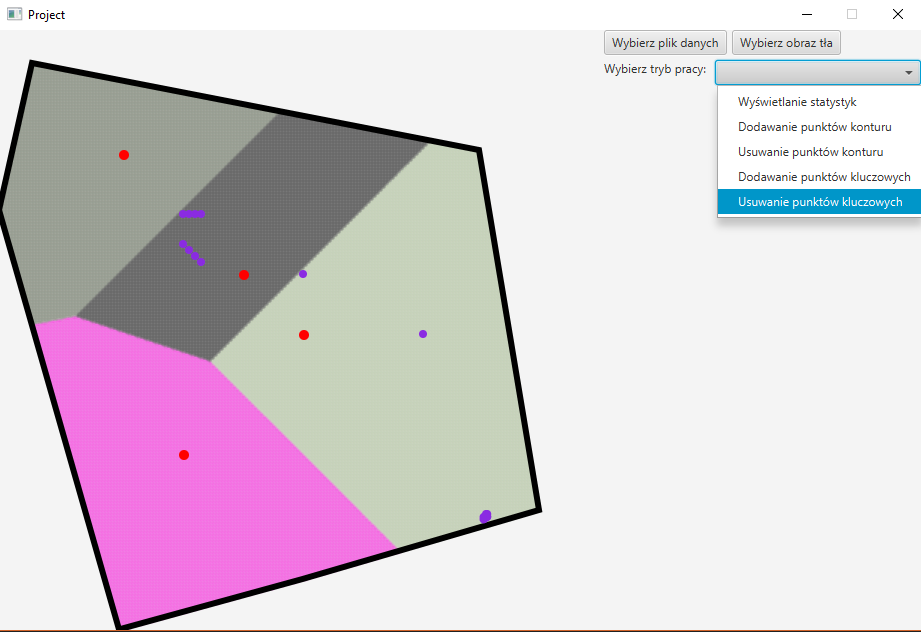
\includegraphics[scale=0.77]{GUI.png}
\end{figure}

\noindent\linia
\section{Zmiany względem specyfikacji}

\noindent\linia
\section{Zmagania z wyznaczaniem optymalnych obszarów}
Szukając sposobu na sprostanie wyzwaniu wyznaczania optymalnych obszarów powstały trzy ścieżki:
\begin{enumerate}
\item Algorytm autorski,
\item Algorytm Fortune'a,
\item Algorytm ostateczny.
\end{enumerate}
\subsection{Algorytm autorski}
Po wstępnym zapoznaniu się z algorytmem Fortune'a, postanowiono poszukać bardziej zrozumiałego rozwiązania.
Tak powstała, przedstawiona poniżej, koncepcja wyznaczania optymalnych obszarów:
\begin{enumerate}
\item Otrzymane punkty kluczowe pogrupować w trójkąty przy pomocy triangulacji S-Hull.
\item Wyznaczyć środki otrzymanych trójkątów (ze wzorów matematycznych).
\item Połączyć środki sąsiadujących trójkątów (sąsiedzi mają wspólny bok).
\item W przypadku braku sąsiada poprowadzić półprostą przez środek trójkąta i środek boku bez sąsiada.
\end{enumerate}
Kiedy podana wyżej koncepcja była gotowa, po bliższych jej oględzinach uznano, że triangulacja w swoim stopniu skomplikowania nie ustępuje algorytmowi Fortune'a.
Biorąc pod uwagę ramy czasowe i pozostałe funkcjonalności, które muszą zostać zrealizowane w przewidzianym czasie, postanowiono dać szansę algorytmowi Fortune'a. Jego skuteczność i poprawność działania są znane historii w przeciwieństwie do ''algorytmu autorskiego'', dlatego postanowiono nie ryzykować pokaźnej straty zasobów czasowych na wypadek nieprawidłowości działania nowo wymyślonego algorytmu.
\subsection{Algorytm Fortune'a}
Praca nad zrozumieniem i implementacją algorytmu Fortune'a trwała do wieczora 31.12 ubiegłego roku.
Udało się zrozumieć jego działanie oraz nakreślić implementację, która znajduje się na gałęzi ''voronoi'' w projektowym repozytorium. Wersja ta działała częściowo poprawnie dla wybranych zbiorów danych. Podjęto próby zlokalizowania źródła błędów, które niestety zakończyły się niepowodzeniem.

Do roboczych testów manualnych użyto klas ''StdDraw'' oraz ''Stopwatch'' (źródło Github), które posłużyły tylko do wyświetlenia efektów pracy nieudanej implementacji algorytmu i nie rościmy sobie do nich praw autorskich. Klasy te nie weszły w skład naszej implementacji i nigdy nie było nawet takich planów. Służyły tylko i wyłącznie do szybkich roboczych testów.

Z nastaniem roku 2019 dokonano bilansu efektów dotychczasowej pracy, poczynionych postępów oraz pozostałych zadań i zestawiono to wszystko z wyznaczonym terminem oddania projektu. W obliczu dwóch tygodni, które pozostały na skończenie projektu (i inne studenckie zobowiązania) oraz przegranej bitwy z tą implementacją (ale nie wojny), podjęto decyzję o porzuceniu tego ambitnego rozwiązania na rzecz pozostałych funkcjonalności. Byliśmy pewni, że prostsza implementacja pozwoli nam spełnić pozostałe wymagania projektu. Chcieliśmy uniknąć sytuacji, w której do tego stopnia skupimy się na wyznaczaniu diagramów Voronoi, że nie starczy nam czasu na pozostałe funkcje programu.

\noindent\linia
\section{Podsumowanie i wnioski}

\noindent\linia
\section{Ocena prowadzenia zajęć}

\noindent\linia

\end{document}



